\subsection*{Exercise 3}
\boldmath
\textbf{Use Corollary $3.8$ (a corollary of Menger’s theorem) to prove the harder direction of Hall’s theorem, that is, given a bipartite graph $G$ with vertex partition $(A,B)$, there is a matching which covers $A$ if for all subsets $X \subseteq A$, $|N(X)| \geq |X|$.\\\linebreak} 
\unboldmath
Corollary 3.8: For any 2 non-adjacent vertices $a,b$ in a graph $G$, there are $k$ internally vertex-disjoint $a-b$ paths if an only if there is no $a-b$ separator $X \subseteq V(G)\setminus \{a, b\}$. \\
\linebreak 
\textbf{Proof} \\
In order for a bipartite graph $G$ to have a matching of $A$, each vertex $v \in A$ must be linked to $\geq 1$ unique vertex $w \in B$ (which also makes $N(A) \geq |A|)$ This is equivalent to finding $|A|$ pairwise disjoint paths. The problem of finding $|A|$ pairwise disjoint paths can be extended further such that we can apply corollary 3.8. \\
\linebreak 
Let $G'$ be obtained by adding two auxiliary vertices $a$ and $b$ such that $a$ is adjacent to all vertices $\in A$ and $b$ is adjacent to all vertices $\in B$. Note that neither $a$ or $b$ are in either of the sets of the bipartition. See fig \ref{fig:bip} for a representation of $G'$. Furthermore, we remove any vertices of degree 0, as these have no impact on whether or not a matching of $A$ can be found. \\
    \begin{figure}[h]
        \centering
        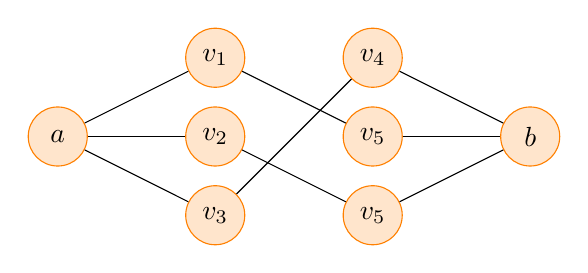
\begin{tikzpicture}
        \tikzset{
            dep/.style={circle,minimum size=0.75cm,fill=orange!20,draw=orange},
            vc/.style={circle, minimum
            size=0.75cm, fill=blue!20, draw=blue},
            c1/.style={-},
            c2/.style={dotted, purple, line width=2},
            c3/.style={dotted, black, line width=2},
            c4/.style={-, out=90, in=145}
            }

            \node[dep] (n1) at (-3,0) {$a$};
            \node[dep] (n2) at (-1,1) {$v_1$};
            \node[dep] (n3) at (-1,0) {$v_2$};
            \node[dep] (n4) at (-1,-1) {$v_3$};
            \node[dep] (n5) at (1,1) {$v_4$};
            \node[dep] (n6) at (1,0) {$v_5$};
            \node[dep] (n7) at (1,-1) {$v_5$};
            \node[dep] (n9) at (3,0) {$b$};

            \draw[c1] (n1) to[above](n2);
            \draw[c1] (n1) to[above](n3);
            \draw[c1] (n1) to[above](n4);
            \draw[c1] (n5) to[above](n9);
            \draw[c1] (n6) to[above](n9);
            \draw[c1] (n7) to[above](n9);
            \draw[c1] (n2) to[above](n6);
            \draw[c1] (n3) to[above](n7);
            \draw[c1] (n4) to[above](n5);
        \end{tikzpicture}
        \caption{Representation of the graph $G'$}
        \label{fig:bip}
    \end{figure}
\linebreak 
Let $|A| = k$, and $|B| \geq |A| \geq k$. The problem of finding if there is a matching of $A$ in $G$ is equivalent to finding if there are at least $k$ pairwise-disjoint paths in $G$ which again is equivalent to finding if there are $k$-internally vertex-disjoints $a-b$ paths in $G'$. \\
\linebreak 
In order to have a matching of $A$, therefore, we must show that any $a-b$ separator has size $\geq k$. Assume, for a contradiction, that there exists a separator $X$ with size $\leq k-1$. We can then identify three cases, all of which give a contradiction: 
\begin{itemize}
    \item $X \subset A$. As we removed any vertices of degree 0, the remaining vertex in $A-X$ will be adjacent to at least one vertex in $B$. We also know that any vertex $\in B$ is adjacent to $b$ and any vertex $\in A$ is adjacent to $a$. Therefore, there must exist an $a-b$ path and so $G'-X$ remains connected. 
    \item We can apply the same reasoning to any set $X \subset B$. (Although $|B-X|$ may be $>$ 1 the same argument applies.)
    \item We take some non-empty $A' \subset A$ and some non-empty $B' \subset B$, s.t. $X = A' \cup B'$ and $|X| \leq k-1$. In this case, we are removing $< k-1$ vertices from both $A$ and $B$ and so we know that at least 1 pair of adjacent vertices $v_1 \in A$ and $v_2 \in B$ remains, and by the same argument as before, $G'-X$ remains connected and we have a contradiction.   
\end{itemize}
In conclusion, we have shown that in order to have a matching of $A$, we need at least $k$-internally disjoint paths, where $k$ = $|A|$, and so $|N(A)| \geq |A|$. \qed